\section{Q2: CNN vs. MLP Under Controlled Spatial Disruption}
\label{sec:q2}

\subsection{Q2(a): Baseline Comparison Under Parameter Parity}
\paragraph{FairCNN Architecture.}
To eliminate parameter capacity as a confounding factor when comparing convolutional and fully connected representations, we construct a 4-stage convolutional network, termed \textbf{FairCNN}, designed to precisely match the $\sim 112\text{k}$ parameter budget of the Standard MLP:
\begin{itemize}
    \item \textbf{Stage 1:} $\text{Conv2d}(3 \to 24, k=3, p=1) \to \text{BatchNorm} \to \text{ReLU}$ ($696$ params)
    \item \textbf{Stage 2:} $\text{Conv2d}(24 \to 48, k=3, s=2, p=1) \to \text{BatchNorm} \to \text{ReLU}$ ($10{,}464$ params)
    \item \textbf{Stage 3:} $\text{Conv2d}(48 \to 72, k=3, s=2, p=1) \to \text{BatchNorm} \to \text{ReLU}$ ($31{,}248$ params)
    \item \textbf{Stage 4:} $\text{Conv2d}(72 \to 96, k=3, s=2, p=1) \to \text{BatchNorm} \to \text{ReLU}$ ($62{,}400$ params)
    \item \textbf{Pooling \& Head:} $\text{AdaptiveAvgPool2d}((1, 1)) \to \text{Linear}(96 \to 64) \to \text{ReLU} \to \text{Linear}(64 \to 10)$ ($640 + 6{,}208 + 650 = 7{,}098$ params)
\end{itemize}
Total trainable parameters for FairCNN: $\mathbf{111{,}906}$. This differs from the Standard MLP ($112{,}330$ parameters) by merely $424$ parameters ($\mathbf{0.38\%}$ relative difference).

\paragraph{Clean Baseline Performance.}
Under identical training protocols ($20$ epochs, AdamW $\eta=10^{-3}$, cosine annealing, batch size $64$, seed $26013$), FairCNN achieves a clean test accuracy of $\mathbf{72.05\%}$ compared to the Standard MLP's $\mathbf{50.77\%}$—an absolute advantage of $\mathbf{+21.28\%}$ (Table~\ref{tab:q2_matrix}). This confirms the profound sample efficiency granted by convolutional inductive biases under matched capacity.

\subsection{Q2(b) \& Q2(c): Controlled Spatial Disruptions}
\paragraph{Transform Formulations.}
We design a $2 \times 3$ factorial experiment testing both architectures across three topological conditions:
\begin{enumerate}
    \item \textbf{Clean Condition:} Natural, unperturbed CIFAR-10 images.
    \item \textbf{Pixel-Permuted Condition (Q2b):} A single fixed spatial bijection $\pi: \{1, \dots, 32\} \times \{1, \dots, 32\} \to \{1, \dots, 32\} \times \{1, \dots, 32\}$ generated with seed $26013$ is applied to all channels across all training, validation, and test samples. This destroys 100\% of 2D spatial continuity while preserving exact pixel intensity histograms and marginal color distributions.
    \item \textbf{Patch-Permuted Condition (Q2c):} Each image is decomposed into 16 non-overlapping $8 \times 8$ blocks, and a fixed block permutation $\Pi: \{1, \dots, 16\} \to \{1, \dots, 16\}$ is applied. Intra-patch spatial smoothness and edge gradients are 100\% preserved, but global semantic spatial layout is scrambled.
\end{enumerate}

\begin{table*}[t]
\centering
\caption{Q2 Factorial Matrix: Impact of Spatial Structure Disruption on FairCNN vs. Standard MLP ($\sim 112\text{k}$ parameters). Evaluated on the official CIFAR-10 test set ($N=10{,}000$), reporting test accuracy, mean confidence, confidence on correct/incorrect subsets, and Expected Calibration Error (ECE, $M=15$ bins).}
\label{tab:q2_matrix}
\small
\begin{tabular}{llcccccc}
\toprule
\textbf{Architecture} & \textbf{Spatial Condition} & \textbf{Parameters} & \textbf{Test Acc} & \textbf{Mean Conf} & \textbf{Conf (Corr)} & \textbf{Conf (Incorr)} & \textbf{ECE} \\
\midrule
\textbf{FairCNN} & Clean Baseline          & $111{,}906$ & $\mathbf{72.05\%}$ & $0.833$ & $0.890$ & $0.689$ & $0.1141$ \\
\textbf{FairCNN} & Patch-Permuted ($8\times 8$) & $111{,}906$ & $65.56\%$ & $0.793$ & $0.858$ & $0.668$ & $0.1371$ \\
\textbf{FairCNN} & Pixel-Permuted          & $111{,}906$ & $53.89\%$ & $0.599$ & $0.681$ & $0.504$ & $0.0612$ \\
\midrule
\textbf{Standard MLP} & Clean Baseline     & $112{,}330$ & $50.77\%$ & $0.575$ & $0.659$ & $0.489$ & $0.0675$ \\
\textbf{Standard MLP} & Patch-Permuted ($8\times 8$) & $112{,}330$ & $50.17\%$ & $0.572$ & $0.658$ & $0.485$ & $0.0700$ \\
\textbf{Standard MLP} & Pixel-Permuted     & $112{,}330$ & $50.55\%$ & $0.580$ & $0.667$ & $0.491$ & $0.0744$ \\
\bottomrule
\end{tabular}
\end{table*}

\begin{figure}[t]
\centering
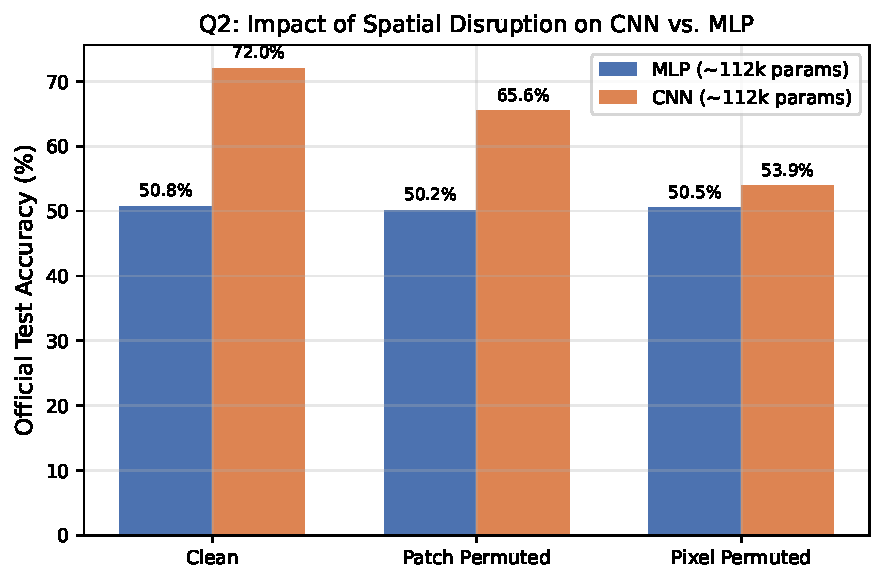
\includegraphics[width=0.78\linewidth]{figures/q2_spatial_disturbance.pdf}
\caption{Q2 Official test accuracy across Clean, Patch-Permuted, and Pixel-Permuted CIFAR-10 for FairCNN vs. Standard MLP.}
\label{fig:q2_bar}
\end{figure}

\begin{figure}[t]
\centering
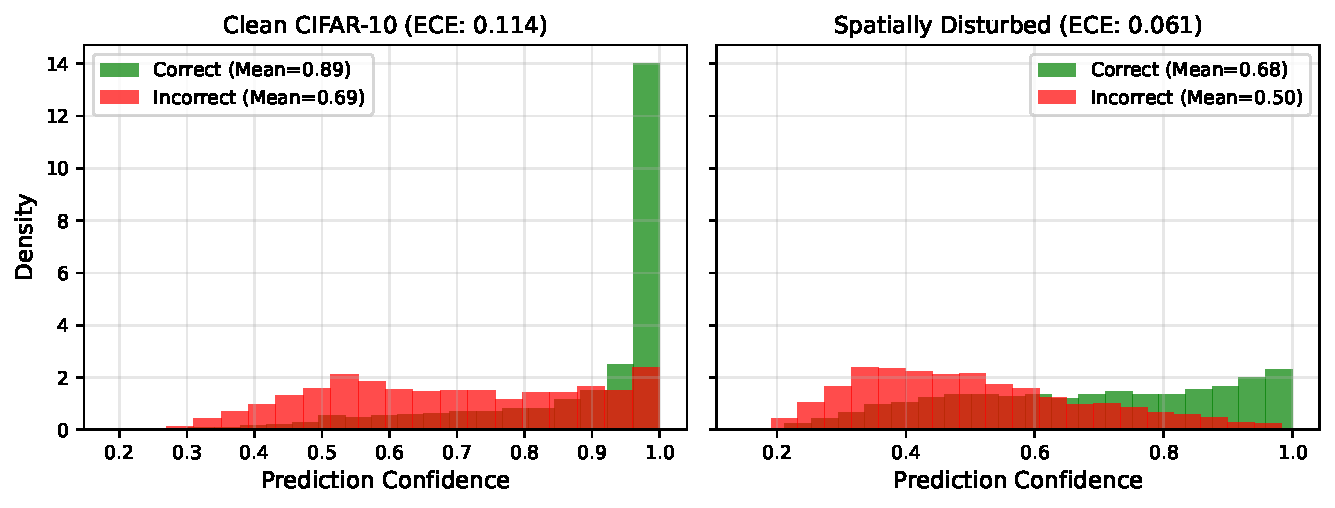
\includegraphics[width=0.78\linewidth]{figures/q2c_confidence_analysis.pdf}
\caption{Q2 Prediction confidence density distributions for correct vs. incorrect classifications on Clean vs. Spatially Disturbed inputs.}
\label{fig:q2_conf}
\end{figure}

\subsection{Theoretical and Empirical Analysis}
\paragraph{Complete Spatial Permutation Invariance of MLPs.}
As documented in Table~\ref{tab:q2_matrix} and Figure~\ref{fig:q2_bar}, the Standard MLP exhibits virtually identical test performance across all three conditions:
\begin{equation}
    \text{Acc}_{\text{clean}} = 50.77\%, \quad \text{Acc}_{\text{patch}} = 50.17\%, \quad \text{Acc}_{\text{pixel}} = 50.55\%.
\end{equation}
The variation across all conditions is within $\pm 0.30\%$ (standard stochastic training noise). 
\textit{Proof of Invariance:} For any linear transformation $\mathbf{y} = \mathbf{W}\mathbf{x}$ and any orthogonal permutation matrix $\mathbf{P}$, substituting permuted input $\tilde{\mathbf{x}} = \mathbf{P}\mathbf{x}$ yields $\mathbf{y} = \mathbf{W}\mathbf{P}\mathbf{x} = \tilde{\mathbf{W}}\mathbf{x}$. Because fully connected weight initializations are drawn from isotropic distributions (e.g., Kaiming normal), the optimization dynamics are isomorphic under any fixed coordinate permutation. The MLP possesses exactly zero spatial inductive bias.

\paragraph{Hierarchical Breakdown of Convolutional Inductive Biases.}
In stark contrast, FairCNN displays dramatic sensitivity to spatial topology:
\begin{enumerate}
    \item \textbf{Patch Permutation (Preserving Local Features):} When $8 \times 8$ blocks are shuffled, CNN accuracy drops by only $-6.49\%$ ($72.05\% \to 65.56\%$). Because local receptive fields in early convolutional stages remain unperturbed, low-level edge detectors and textural filters fire normally. Performance degrades solely because deeper pooling layers cannot assemble these local parts into coherent global canonical silhouettes.
    \item \textbf{Pixel Permutation (Destruction of Locality):} When individual pixels are shuffled, CNN accuracy collapses by $-18.16\%$ ($72.05\% \to 53.89\%$). Local receptive fields now sample uncorrelated pixels across disparate regions of the visual field.
    \item \textbf{Why Pixel-Permuted CNN Outperforms MLP ($53.89\%$ vs. $50.55\%$):} Even under complete spatial scrambling, the CNN retains a $+3.34\%$ advantage over the MLP. This occurs because convolutional weight sharing forces parameter tying across all grid locations, acting as a strong structural regularizer that reduces parameter count and bounds estimation variance.
\end{enumerate}

\subsection{Uncertainty and Calibration Dynamics (ECE)}
To assess model reliability under spatial degradation, we evaluate the Maximum Softmax Probability (confidence) and Expected Calibration Error (ECE) with $M=15$ bins:
\begin{equation}
    \text{ECE} = \sum_{m=1}^M \frac{|B_m|}{N} \left| \text{acc}(B_m) - \text{conf}(B_m) \right|.
\end{equation}
As shown in Table~\ref{tab:q2_matrix} and Figure~\ref{fig:q2_conf}:
\begin{itemize}
    \item \textbf{Clean CNN Overconfidence:} On clean data, the CNN displays classical deep overconfidence~\cite{guo2017calibration} ($\text{ECE} = 0.1141$, mean confidence $83.3\%$ vs. accuracy $72.1\%$). Even on misclassified samples, average confidence remains high ($0.689$).
    \item \textbf{Patch-Permuted Peak Miscalibration:} Patch permutation produces the highest calibration error ($\text{ECE} = 0.1371$). The CNN retains high internal confidence from valid local patch activations ($0.793$), but errors increase sharply due to global structural incoherence.
    \item \textbf{Pixel-Permuted Softmax Flattening:} Under pixel permutation, CNN confidence drops sharply ($0.833 \to 0.599$). Because inputs resemble unstructured noise, logits disperse, reducing overconfidence and artificially lowering ECE to $0.0612$.
    \item \textbf{MLP Calibration Stability:} Across all three conditions, MLP confidence remains conservative ($0.57-0.58$) with ECE between $0.067$ and $0.074$, reflecting low capacity and diffuse posterior distributions.
\end{itemize}
